\documentclass[runningheads]{llncs}

\usepackage{amssymb}
\usepackage{amsmath}
%% The amsthm package provides extended theorem environments

% \usepackage{amsthm}
% AM commented out because it clashes with proof, etc

%% The lineno packages adds line numbers. Start line numbering with
%% \begin{linenumbers}, end it with \end{linenumbers}. Or switch it on
%% for the whole article with \linenumbers.
\usepackage{lineno}

%% Use package enumitem to align enumeration and itemization
\usepackage{enumitem}
\usepackage{listings}
\usepackage{courier}           % for the courier font (optional)
\usepackage{multicol}          % for two equations side by side
\usepackage[justification=centering]{caption}
\usepackage{xcolor}
\usepackage{stmaryrd}
\usepackage{hyperref}
%\usepackage{cleveref}
\usepackage{hieroglf}
\usepackage{scalerel}
\usepackage{tikz}
\usepackage{pgfplots}


\hypersetup{ % play with these to change the look of hyperlinks
    colorlinks=true,
    linkcolor=black,
    filecolor=magenta,
    urlcolor=blue,
    citecolor=black
}

\newcommand{\coq}{\scalebox{.6}{\textpmhg{\Ha}}}

% required by LNCS
\renewcommand\UrlFont{\color{blue}\rmfamily}

\colorlet{red}{red!80!black}
\colorlet{green}{green!50!black}

%% NEW COMMANDS =============================================

\lstdefinestyle{myStyle}{
%	language=Coq,
    keywords={Inductive,Require,Import,Definition,Fixpoint,match,with,end,let,in,fix},
	basicstyle=\normalfont\footnotesize\tt,
    keywordstyle=\color{green}, % Blue clashes with the cyan links. Change if you want.
	stepnumber=1,
	tabsize=2,
    numbers=none,
    numberstyle=\tiny,
    numbersep=5pt,
	showspaces=false,
    escapechar=`,
	showstringspaces=false
}
%basicstyle=\fontsize{10}{11}\selectfont\ttfamily,

\lstdefinestyle{myTinyStyle}{
%   language=Coq,
    keywords={Inductive,Require,Import,Definition,Fixpoint,match,with,end,let,in,fix},
    basicstyle=\normalfont\fontsize{8.2}{8.5}\tt,
    keywordstyle=\color{green}, % Blue clashes with the cyan links. Change if you want.
    stepnumber=1,
    tabsize=2,
    numbers=none,
    numberstyle=\tiny,
    numbersep=5pt,
    showspaces=false,
    escapechar=`,
    showstringspaces=false
}

\lstset{style=myStyle}
\makeatletter
\newlength{\@mli}
\newcommand{\mli}[1]{%
  \settowidth{\@mli}{\lstinline/#1/}
  \hspace{-.5ex}\begin{minipage}[t]{\@mli}\lstinline/#1/\end{minipage}}
\makeatother
\newcommand{\li}[1]{\ifmmode\mbox{\mli{#1}}\else\mbox{\lstinline/#1/}\fi}

\newcommand\hide[1]{}

\newenvironment{centermath}
 {\begin{center}$\displaystyle}
 {$\end{center}}

\renewcommand{\note}[2][polish]{{\color{red} #2}{\marginpar{\tiny \color{blue} #1}}}
\renewcommand{\implies}{\Rightarrow}
\renewcommand{\iff}{\Leftrightarrow}

\title{A Machine-Checked C Implementation of Dijkstra's Shortest Path Algorithm}
\subtitle{Short Paper}
\titlerunning{Machine-Checked Dijkstra}
%optional, please use if title is longer than one line

\begin{document}

\author{Anshuman Mohan \and Aquinas Hobor}
\authorrunning{A. Mohan, A. Hobor}

%\author{Linh Tran \and Anshuman Mohan \and Aquinas Hobor}
%\authorrunning{L. Tran, A. Mohan, A. Hobor}
% First names are abbreviated in the running head.
% If there are more than two authors, 'et al.' is used.
%
\institute{National University of Singapore \\
\email{\{mohan,hobor\}@comp.nus.edu.sg}}


\maketitle
%\begin{frontmatter}

%% Title, authors and addresses

%% use the tnoteref command within \title for footnotes;
%% use the tnotetext command for theassociated footnote;
%% use the fnref command within \author or \address for footnotes;
%% use the fntext command for theassociated footnote;
%% use the corref command within \author for corresponding author footnotes;
%% use the cortext command for theassociated footnote;
%% use the ead command for the email address,
%% and the form \ead[url] for the home page:

%% \tnotetext[label1]{}
%% \author{Name\corref{cor1}\fnref{label2}}
%% \ead{email address}
%% \ead[url]{home page}
%% \fntext[label2]{}
%% \cortext[cor1]{}
%% \address{Address\fnref{label3}}
%% \fntext[label3]{}

%% use optional labels to link authors explicitly to addresses:
%% \author[label1,label2]{}
%% \address[label1]{}
%% \address[label2]{}

%\author{}

%\address{}


\begin{abstract}
\vspace{-2em}
We report on a machine-checked proof of correctness for 
Dijkstra’s one-to-all shortest path algorithm. 
Unlike previous work, we use classic textbook code written in C.
Our C code is executable and realistic but also has 
real-world complications. 
We prove full functional correctness, and not just program safety.
We show that Dijkstra’s algorithm suffers from potential overflow issues. 
The precise bound is nontrivial: we show that the intuitive guess 
fails, and provide a workable refinement.

\keywords{Dijkstra \and verification \and Coq}
\end{abstract}

%\end{frontmatter}

%% \linenumbers

%% main text

% \section{Overview}
% \label{sec: overview}
% 
Figure~\ref{fig:decorated} shows the code and proof
sketch of Dijkstra's algorithm.  Our code is implemented exactly
as suggested by CLRS~\cite{clrs} so we refer readers there for a
general discussion of the algorithm.
The adjacency-matrix-represented graph $\gamma$ of \texttt{SIZE} vertices
is passed as the parameter \texttt{graph} along with the source vertex \texttt{src}
and two allocated arrays \texttt{dist} and \texttt{prev}.
The details of the spatial predicates $\mathsf{array}(x,\vec{v})$, connecting an array pointer $x$ with its contents $\vec{v}$, and the internals of the priority
queue $\mathsf{PQ}$ are unexciting.  Our spatial graph predicate is more interesting in
that it nests arrays and connects the concrete memory values to an abstract mathematical
graph $\gamma$, which in turn exposes an interface in the language of graph theory
(vertices, edges, labels, etc.).

\begin{equation*}
\begin{split}
\m{list\_addr} ((\m{block}, \m{offset}), \m{index}) &\defeq
  (\m{block}, \m{offset} + (\m{index} \times \texttt{sizeof}(\texttt{int}) \times \texttt{SIZE})) \\
\p{list\_rep}(\gamma, \m{i}, \m{base\_ptr}) &\defeq \mathsf{array}(\mathsf{graph2matrix}(\gamma)[\m{i}], \m{list\_addr}(\m{base\_ptr}, \m{i})) \\
\vspace{1em}
\p{graph\_rep}(\gamma, \m{g\_addr}) &\defeq \underset{\m{v} \in \gamma}{\bigstar} \m{v}  \mapsto\p{list\_rep}(\gamma, \m{v}, \m{g\_addr})
\end{split}
\end{equation*}

In general these spatial representations are simple enough that they pose no special
challenge in the proof and so we will not focus on issues such as \emph{e.g.}~making
sure an array dereference is in bounds in our discussion below.

The key to the verification is the pure part of the loop
invariants on lines~\ref{code:whileinv} and~\ref{code:forinv}.  The \texttt{while} invariant $\m{dijk\_correct}(\gamma, \texttt{src}, \m{prev}, \m{dist}, \m{priq})$ has three parts:
\[
\begin{array}{l}
\forall \m{dst}.~\texttt{0} \le \m{dst} < \texttt{SIZE} -> \m{inv\_popped}(\gamma, \texttt{src}, \m{prev}, \m{dist}, \m{priq}, \m{dst}) /| \null \\
\hspace{11em}\m{inv\_unpopped}(\gamma, \texttt{src}, \m{prev}, \m{dist}, \m{priq}, \m{dst}) /| \null \\
\hspace{11em}\m{inv\_unseen}(\gamma, \m{prev}, \m{dist}, \m{priq}, \m{dst})
\end{array}
\]
A destination vertex $\m{dst}$ falls into one of three
categories:
\begin{enumerate}
\item $\m{inv\_popped}$: $\m{dst}$ has been fully processed, and has been
popped from the priority queue.
A globally optimal path from $\texttt{src}$
to $\m{dst}$ exists, the cost of this path is logged in
the \texttt{dist} array, and all the vertices visited by the path are also popped.
Further, the links of this path are logged in the \texttt{prev} array.
\item $\m{inv\_unpopped}$: $\m{dst}$ is reachable in
one hop from a ``\emph{mom}'' vertex, which is itself popped.
This route is locally optimal: we cannot
improve the cost by going via a \emph{different} popped vertex.
The \texttt{prev} array logs
\emph{mom} as the best-known way to reach $\m{dst}$, and the \texttt{dist}
array logs the cost of the path via \emph{mom} as the best-known cost.
\item $\m{inv\_unseen}$: no path is currently known from $\texttt{src}$ to $\m{dst}$.
\end{enumerate}
After popping the lowest-cost vertex in line~\ref{code:pop}, we reach the invariant of
the \texttt{for} loop $\m{dijk\_correct\_weak}(\gamma, \texttt{src}, \m{prev}, \m{dist}, \m{priq}, \texttt{i}, \texttt{u})$:
\[
\begin{array}{l}
\forall \m{dst}.~\texttt{0} \le \m{dst} < \texttt{SIZE} -> \m{inv\_popped}(\gamma, \m{src}, \m{prev}, \m{dist}, \m{priq}, \m{dst}) /| \null \\
\hspace{11em}\m{inv\_unseen}(\gamma, \m{prev}, \m{dist}, \m{priq}, \m{dst}) /| \null \\
\forall \m{dst}.~\texttt{0} \le \m{dst} < \texttt{i} -> \m{inv\_unpopped}(\gamma, \m{src}, \m{prev}, \m{dist}, \m{priq}, \m{dst}) /| \null \\
\forall \m{dst}.~\texttt{i} \le \m{dst} < \texttt{SIZE} -> \m{inv\_unpopped\_weak}(\gamma, \m{src}, \m{prev}, \m{dist}, \m{priq}, \m{dst}, \texttt{u})
\end{array}
\]
We now have four cases:
\begin{enumerate}
\item $\m{inv\_popped}$: $\m{dst}$ has been fully processed, and has been
popped from the priority queue.  For all popped vertices \emph{except for} \texttt{u}
this is trivial from $\m{dijk\_correct}$; for \texttt{u} itself we reach the heart of Dijkstra's correctness: the cost to the fringe vertex with minimum cost cannot be further improved.  The associated entailment is not trivial.
\item $\m{inv\_unseen}$: no path is currently known from $\texttt{src}$ to $\m{dst}$.  Trivially holds from $\m{dijk\_correct}$.
\item $\m{inv\_unpopped}$ (less than \texttt{i}): $\m{dst}$ is reachable in
one hop from a ``\emph{mom}'' vertex, which is itself popped.  Initially this is trivial since $\texttt{i}=0$ and we restore it as \texttt{i} climbs by updating costs when they can be improved in line~\ref{code:update}.
\item $\m{inv\_unpopped\_weak}$ (between than \texttt{i} and \texttt{SIZE}): ANSHUMAN
\end{enumerate}
The formal definitions for the above predicates, and the key subdefinitions upon which they rely, can be found in appendix~\ref{sec:apx}.

\hide{

While loop's invariant, which is stated on line
and explained further in Figure~\ref{fig:defns}.


This three-part invariant is trivially true before the while loop.
On line~\ref{code:pop}, the minimal vertex from the priority queue is popped,
thus breaking the invariant.

First, we must show that the minimal vertex $\m{u}$
obeys $\m{inv\_popped}$. \emph{i.e.}, show that the locally
optimal path to $\m{u}$ is, in fact, globally optimal.
This comes from blah blah blah

\newcommand{\s}{11}
\begin{figure}[htbp]
  \centering
  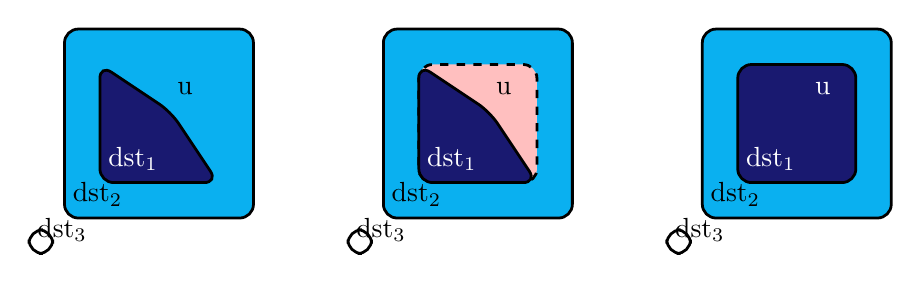
\begin{tikzpicture}[x=0.3cm, y=0.3cm,
      popped/.style={rounded corners=5pt, line width=1pt, draw, fill=MidnightBlue},
      fringe/.style={rounded corners=5pt, line width=1pt, draw, fill=ProcessBlue},
      popping/.style={rounded corners=5pt, line width=1pt, draw, dashed, fill=pink},
      unseen/.style={rounded corners=5pt, line width=1pt, draw}]
    \draw[unseen] (0,0) -- (\s,0) -- (\s,\s) -- (0,\s) -- cycle;
    \draw[fringe] (1.5,1.5) -- (9.5,1.5) -- (9.5,9.5) -- (1.5,9.5) -- cycle;
    \draw[popped] (3,3) -- (8,3) -- (6,6) -- (3,8) -- cycle;
    \node at (1.4,1) {dst$_3$};
    \node at (2.9,2.5) {dst$_2$};
    \node at (4.4,4) {\color{white}dst$_1$};
    \node at (6.6,7) {u};
    \tikzset{shift={(13.5,0)}}

    \draw[unseen] (0,0) -- (\s,0) -- (\s,\s) -- (0,\s) -- cycle;
    \draw[fringe] (1.5,1.5) -- (9.5,1.5) -- (9.5,9.5) -- (1.5,9.5) -- cycle;
    \draw[popping] (3,3) -- (8,3) -- (8,8) -- (3,8) -- cycle;
    \draw[popped] (3,3) -- (8,3) -- (6,6) -- (3,8) -- cycle;
    \node at (1.4,1) {dst$_3$};
    \node at (2.9,2.5) {dst$_2$};
    \node at (4.4,4) {\color{white}dst$_1$};
    \node at (6.6,7) {u};

    \tikzset{shift={(13.5,0)}}

    \draw[unseen] (0,0) -- (\s,0) -- (\s,\s) -- (0,\s) -- cycle;
    \draw[fringe] (1.5,1.5) -- (9.5,1.5) -- (9.5,9.5) -- (1.5,9.5) -- cycle;
    \draw[popped] (3,3) -- (8,3) -- (8,8) -- (3,8) -- cycle;
    \node at (1.4,1) {dst$_3$};
    \node at (2.9,2.5) {dst$_2$};
    \node at (4.4,4) {\color{white}dst$_1$};
    \node at (6.6,7) {\color{white}u};
  \end{tikzpicture}
  \caption{Popping $\m{u}$}
\end{figure}

Next, we must account for the ripple effect that popping
$\m{u}$ could have had on the other vertices.
In particular, it is possible that a vertex obeying $\m{inv\_unpopped}$ can
improve its cost via $\m{u}$, and that an unreachable vertex
obeying $\m{inv\_unseen}$ can now be reached via $\m{u}$.
The for loop repairs these breakages by
checking if a path via $\m{u}$ is an improvement for such vertices, and, if so,
edits both arrays and the priority queue as seen on line~\ref{code:update}.

The for loop's invariant is similar to that of the while loop---$\m{inv\_unseen}$
and $\m{inv\_popped}$ are preserved as-is, modulo the popping of
$\m{u}$ as discussed above. The key edit is in $\m{inv\_unpopped}$. blah blah blah

}



\begin{figure}[t]

\begin{lstlisting}[mathescape=true,showlines=true]
void dijkstra (int **g, int src, int *dist,
               int *prev, int size, int inf {
$\color{OliveGreen}//~\braces{\p{AdjMat}(\texttt{g},\gamma) *
\mathsf{array}(\texttt{dist}, \_) * \mathsf{array}(\texttt{prev}, \_)}$
 Item* temp = (Item*) mallocN(sizeof(Item));
 int* keys = mallocN (size * sizeof (int));
 PQ* pq = pq_make(size); int i, j, u, cost;
 for (i = 0; i < size; i++)
 { dist[i] = inf; prev[i] = inf; keys[i] = pq_push(pq,inf,i); } $\label{code:assigninf}$
 dist[src]= 0; prev[src]= src; pq_edit_priority(pq,keys[src],0);
 while (pq_size(pq) > 0) {
$\color{OliveGreen}//~\braces{{\color{red}\exists \m{dist}, \m{prev}, \m{popped}, \m{heap}}.~\p{AdjMat}(\texttt{g},\gamma) * {\color{red}\p{PQ}(\texttt{pq},\m{heap})} *
{\color{red}\mathsf{Item}(\texttt{temp}, \_)} * \null \\
\mathsf{array}(\texttt{dist},{\color{red}\m{dist}}) *
\mathsf{array}(\texttt{prev}, {\color{red}\m{prev}}) *
{\color{red}\mathsf{array}(\texttt{keys}, \m{keys}}) /| \null \\
{\color{red}\m{linked\_correctly}(\gamma, \m{heap}, \m{keys}, \m{dist}, \m{popped})} /| \null \\
{\color{red}\m{dijk\_correct}(\gamma,\texttt{src},\m{popped},\m{prev},\m{dist})}}$ $\label{code:whileinv}$
  pq_pop(pq, temp); u = temp->data; $\label{code:pop}$
  for (i = 0; i < size; i++) {
$\color{OliveGreen}//~\braces{{\color{red}\exists \m{dist'}, \m{prev'}, \m{heap'}}.~\p{AdjMat}(\texttt{g},\gamma) * \p{PQ}(\texttt{pq},{\color{red}\m{heap'}}) * \null \\
\mathsf{array}(\texttt{dist},\m{\color{red}dist'}) *
\mathsf{array}(\texttt{prev}, \m{\color{red}prev'}) *
\mathsf{array}(\texttt{keys}, \m{keys}) * \null \\
\mathsf{Item}(\texttt{temp}, \m{\color{red}(\texttt{keys[u]}, \texttt{dist[u]}, \texttt{u})}) /|
\m{\color{red}min(\texttt{dist[u]}, \m{heap'})} /| \null \\
{\m{linked\_correctly}(\gamma, \m{\color{red}heap'}, \m{keys}, \m{\color{red}dist'},
{\color{red}\m{popped} \uplus \{\texttt{u}\}})} /| \null \\
{\color{red}\m{dijk\_correct\_weak}({\color{OliveGreen}\gamma, \texttt{src}}, \m{popped} \uplus \{\texttt{u}\}, \m{prev'}, \m{dist'}, \texttt{i}, \texttt{u})}}$ $\label{code:forinv}$
   cost = getCell(g, u, i); $\label{code:cost}$
   if (cost < inf) {
    if (dist[i] > dist[u] + cost) { $\label{code:overflow}$
     dist[i] = dist[u] + cost; prev[i] = u; $\label{code:update1}$
     pq_edit_priority(pq, keys[i], dist[i]); $\label{code:update2}$
  }}}} $\color{OliveGreen}//~\braces{{\color{red}\exists \m{dist''}, \m{prev''}}.~\p{AdjMat}(\texttt{g},\gamma) * \p{PQ}(\texttt{pq},\m{\color{red}\emptyset}) * {\mathsf{Item}(\texttt{temp}, {\color{red}\_})} * \null \\
 \mathsf{array}(\texttt{dist},\m{\color{red}dist''}) *
 \mathsf{array}(\texttt{prev}, \m{\color{red}prev''}) *
 \mathsf{array}(\texttt{keys}, \m{keys}) /| \null \\
{\color{red}\forall \m{dst}.~0 \le \m{dst} < \texttt{size} -> \m{inv\_popped}}(\gamma, \m{src}, {\color{red}\m{\gamma.V}, \m{prev''}, \m{dist''}, \m{dst}})}$ $\label{code:end}$
 freeN (temp); pq_free (pq); freeN (keys); return; }
\end{lstlisting}
\vspace{-1em}
\caption{C code and proof sketch for Dijkstra's Algorithm.}
\vspace{-1em}
\label{fig:decorated}
\end{figure}



\hide{
$\color{OliveGreen}//~\braces{{\color{red}\exists \m{dist''}, \m{prev''},\m{heap''}}.~\p{AdjMat}(\texttt{g},\gamma) * \p{PQ}(\texttt{pq},\m{\color{red}heap''}) *
  \mathsf{array}(\texttt{dist},\m{\color{red}dist''}) * \null \\
  \mathsf{array}(\texttt{prev}, \m{\color{red}prev''}) *
  \mathsf{array}(\texttt{keys}, \m{keys}) *
  \mathsf{Item}(\texttt{temp}, \m{(\texttt{keys[u]}, \texttt{dist[u]}, \texttt{u})} /| \null \\
  \m{min(\texttt{dist[u]}, \m{heap'})} /|
  {\color{red}\m{heap''} = \m{heap'} [\texttt{keys[i]} \mapsto (\texttt{dist[i]},\texttt{i})]} /| \null \\
  {\m{\color{red}dijk\_correct}(\gamma, \texttt{src}, \m{popped'}, \m{\color{red}prev''}, \m{\color{red}dist''})}}$ $\label{code:caughtup}$
}




%% If you have bibdatabase file and want bibtex to generate the
%% bibitems, please use
%%
%\bibliographystyle{plainurl}% the mandatory bibstyle

\bibliographystyle{splncs04}
\bibliography{dijkstra}

%% The Appendices part is started with the command \appendix;
%% appendix sections are then done as normal sections
\appendix
% 
\appendix

{\color{magenta}
\section{Simplifying ramification entailments}
After applying \infrulestyle{Solve Ramify-PQ}, it is often desirable to break the ramification entailment into smaller disjoint pieces before trying to solve it directly.
One common case is to ``frame out'' an unneeded part of the global state:
\[
\infrule{Frame Ramify-Q}
{G_1 \vdash L_1 * \forall x.~ (L_2 --* G_2)}  
{G_1 * F \vdash L_1 * \forall x.~ \big(L_2 --* (G_2 * F)\big) }
{\begin{array}{c}F \text{ ignores} \\ \MV(c) \cup \{x\} \end{array}} \qquad \qquad \qquad
\]
In fact \infrulestyle{Frame Ramify-Q} is a consequence of the more general \[
\infrule{Split Ramify-Q}
{G_1 \vdash L_1 * \big(\forall x.~ (L_2 --* G_2)\big) \! \! \! \! \\
 G_1' \vdash L_1' * \big(\forall x.~ (L_2' --* G_2')\big) }
{G_1 * G_1' \vdash L_1 * L_1' * \Big(\forall x.~ \big((L_2 * L_2') --* (G_2 * G_2')\big)\Big)} {}
\]
In general the strategy is to apply \infrulestyle{Frame Ramify-P} and \infrulestyle{Split Ramify-P} until the ramification entailments are as small as they can be (while remaining true!) before using \infrulestyle{Solve Ramify-P} on the remaining ``atoms''.

The situation is unfortunately a little messier when the postconditions contain existential quantifiers.

\[\text{UNSOUND-RAM-Q-SPLIT}\]
\Rule{}
{G_1 \vdash L_1 * (\exists x, L_1' (x) --* \exists x, G_1'(x)) \\
G_2 \vdash L_2 * (\exists x, L_2' (x) --* \exists x, G_2'(x)) \\}
{G_1 * G_2 \vdash L_1 * L_2 * (\exists x, L_1'(x) * L_2'(x) --* \exists x, G_1'(x) * G_2'(x)) }


\[
\infrule{Ramify-Q}
{\{ L \} ~ c ~ \{\exists x.~ L' \} \\
 G \vdash L * \big(\forall x.~ (L' --* G')\big)}
{\{ G \} ~ c ~ \{ \exists x.~G' \}}{}
\]

}


\section{Junk}
{\color{magenta} Universally-quantified metavariables can appear free in the predicates to make further connections.
Assuming that the abstracted pre- and postconditions $A$, $B$, $C$, and $D$ above all use \li{x}, we proceed
as follows.  First we introduce a new fresh metavariable $x$ whose value will be equal to \li{x} after the localization, and then choose $F \stackrel{\Delta}{=} [\li{x} |-> x] (C -* D)$, that is we substitute the program
variable \li{x} for the metavariable $x$.  Since we have substituted away \li{x}, $F$ ignores it and so we satisfy the side condition on \infrulestyle{Solve Ramify-P}.  We then must strengthen $C$ into $C' \stackrel{\Delta}{=} C /| \li{x} = x$ to make the connection at the appropriate program point.  Now we are left with the entailments
\[
\begin{array}{lcl}
\li{x} = 5 /| A & |- & (\li{x} = 5 /| B) * F \\
F & |- & (\li{x} = 6 /| C') -* (x = 6 /| D)
\end{array}
\]
To further relate the earlier and later values of \li{x} in $F$ we can introduce a second fresh $x'$ and use $B' \stackrel{\Delta}{=} B /| \li{x} = x'$.
}

The \infrulestyle{Ramify} rule is sound but interacts poorly with modified program variables (as in lines~\ref{code:markbeforetripleramify}--\ref{code:markaftertripleramify} of Figure~\ref{fig:markgraph}) {\color{magenta} and
localized existentials (as in lines~\ref{code:beforemarkl}--\ref{code:aftermarkl})}.  Both of these limitations are annoying enough in paper proofs and graduate to major headaches in mechanized ones.  Happily, we show how to overcome both limitations in \S\ref{sec:freevars} and \S\ref{sec:existentials}, respectively, by presenting new variants of \infrulestyle{Ramify}.  Our notation carries over without significant change: just use the new rules to enable the more general ramification entailments they permit.
%When in doubt the most general rule, \infrulestyle{Ramify-PQ} from \S\ref{sec:existentials}, implies all of the others.

\section{More junk}
\hide{
\section{Ramification Rules}


\Rule{Frame  }
{\{ P \} c \{Q \} \\
  F \text{ is stable w.r.t. } \MV(c)\\}
 {\{P * F \} c \{ Q * F \}}

\Rule{Ramification   }
{\{ L \} c \{L' \} \\
 G \vdash L * (L' -* G') \\
 (L' -* G') \text{ is stable w.r.t. } \MV(c)\\}
{\{ G \} c \{ G' \}}

\Rule{Ramification-P }
{\{ L \} c \{L' \} \\
 G \vdash L * \Box^{\llbracket c \rrbracket} (L' -* G') \\}
{\{ G \} c \{ G' \}}

\subsection{P for Pure Facts}

Separation logic has been mechanized by many projects CITE CITE CITE.
In many of them, like VST and Charge!, expressing the value of a local
variable (a variable stored in stack) is a pure fact rather than a
spatial fact. Because the side condition of ramification rule requires $(L' -* G')$ to be stable w.r.t. modified local variables in $c$\footnote{In previous papers, the side conditions of Frame rule and ramification rule are usually expressed as ``$\FV(F) \cap \MV(c) = \emptyset$'' and ``$\FV(L' -* G') \cap \MV(c) = \emptyset$''. The side conditions used in this paper are equivalent with typical ones if the semantic interpretation of $\FV$ is used. All the previous mentioned projects takes semantic interpretation instead of syntactical interpretation.}, it is almost impossible to apply ramification rule in any practical situations in these systems. In this paper, we present a pure-facts-related rule (we call it ramification-P rule, or just P rule, in the rest of this paper) such that it is sound and practical in the most general setting of separation logics.

The primary ramification rule is essentially an application of the frame rule using $(L' -* G')$ as frame.
Thus, the key point of handling pure facts is to find a legal frame even if $(L' -* G')$ is not stable w.r.t. $\MV(c)$. This frame is $\Box^{\llbracket c \rrbracket} (L' -* G')$ in ramification-P rule.
\begin{eqnarray*}
m \models \Box^R P &  \Leftrightarrow  & \forall m', \text{ if } m\xrightarrow{R}m' \text{ then } m' \models P \\
m \xrightarrow{\llbracket c \rrbracket} m' & \Leftrightarrow &   \text{$m$ and $m'$ coincide everywhere} \\
&& \text{except $\MV(c)$} \\
P \text{ is stable} &  \Leftrightarrow  & \forall m \ m',  \text{if $m$ and $m'$ coincide everywhere} \\
\text{w.r.t. $S$} && \text{except $S$, then $m \models P$ iff $m' \models P$}
\end{eqnarray*}

Here, $\Box$ represents the necessity modal operator. The formula $\Box^{\llbracket c \rrbracket} (L' -* G')$ says, it is true on a state $m$ if and only if for any state $m'$, if $m$ and $m'$
coincide everywhere except on the variables modified by $c$, then $(L' -* G')$ is true on $m'$.

Based on the combination frame rule, consequence rule and three basic facts below, we can immediate prove ramification-P rule.
\begin{quotation}
(a) $\Box^{\llbracket c \rrbracket} (L' -* G')$ is stable w.r.t. $\MV(c).$\footnote{This can be proved directly from the definition of $\llbracket c \rrbracket$ and stability, and the fact that $\llbracket c \rrbracket$ is an equivalence relation.}

(b) $G \vdash L * \Box^{\llbracket c \rrbracket} (L' -* G')$. (Assumption)

(c) $L' *  \Box^{\llbracket c \rrbracket} (L' -* G') \vdash G'$. \footnote{When $R$ is reflexive, T-Axiom of modal logic is sound, i.e. for any $P$, $\Box^R P \vdash P$. As $\llbracket c \rrbracket$ is reflexive, we know the fact that $\Box^{\llbracket c \rrbracket} (L' -* G') \vdash L' -* G'$, which is immediate followed by $L' *  \Box^{\llbracket c \rrbracket (L' -* G')} \vdash G'$.}
\end{quotation}

\subsection{Establish the Assumption Entailment of P Rule}

It is well-known that the proof theory with magic wand is already complicated, so generally speaking, it will not be a easy task to prove an entailment with magic wand together with modality. However, people need to prove an entailment with form
\begin{equation}G \vdash  L * \Box^R (L' -* G') \label{eqn:Passu} \end{equation}
at first when applying ramification-P rule. Luckily, this special form makes the task simpler.

First of all, SOLVE-RAM-P rule can turn the proof goal into two wand-free and modality-free entailments. Specifically, people only need to find an $R$-stable predicate $F$, such that $G \vdash L * F$ and $F * L' \vdash G'$ are both true.

SOLVE-RAM-P alone is not a satisfactory proof theory because in that case using P rule would have no different from using frame rule directly. The key point here is that, an entailment with form \ref{Passu} can be proved in a modularized way. For primary ramification rule, CITE proposed two proof rule, RAM-FRAME and RAM-SPLIT\footnote{\Rule{RAM-FRAME }
{G \vdash L * (L' -* G') \\
F \text{ is stable w.r.t. } \MV(c) \\}
{G * F \vdash L * (L' -* G' * F) }

\Rule{RAM-SPLIT }
{G_1 \vdash L_1 * (L_1' -* G_1') \\
G_2 \vdash L_2 * (L_2' -* G_2') \\}
{G_1 * G_2 \vdash L_1 * L_2 * (L_1' * L_2' -* G_1' * G_2') }
}, to divide an entailment with form $G \vdash L * (L' -* G')$ into small pieces. When it comes to ramification-P rule, two corresponding proof rules, RAM-P-FRAME and RAM-P-SPLIT are still sound.

\Rule{SOLVE-RAM-P }
{G \vdash L * F\\
F * L' \vdash G' \\
F \text{ is stable w.r.t. } \MV(c) \\}
{G \vdash L * \Box^{\llbracket c \rrbracket} (L' -* G') }

\Rule{RAM-P-FRAME }
{G \vdash L * \Box^{\llbracket c \rrbracket} (L' -* G') \\
F \text{ is stable w.r.t. } \MV(c) \\}
{G * F \vdash L * \Box^{\llbracket c \rrbracket} (L' -* G' * F) }

\Rule{RAM-P-SPLIT }
{G_1 \vdash L_1 * \Box^{\llbracket c \rrbracket} (L_1' -* G_1') \\
G_2 \vdash L_2 * \Box^{\llbracket c \rrbracket} (L_2' -* G_2') \\}
{G_1 * G_2 \vdash L_1 * L_2 * \Box^{\llbracket c \rrbracket} (L_1' * L_2' -* G_1' * G_2') }

To conclude, if $L'$ and $G'$ are two separating conjunctions of a bunch of atomic predicates, RAM-P-FRAME and RAM-P-SPLIT can establish \ref{Passu} from entailments with the same form but smaller size. Atomic sized entailments can be proved using SOLVE-RAM-P. They are usually general purposed entailments and do not need to be proved for every single program. In section \ref{vst}, we will see examples of this approach for real programs.

\subsection{Q for Quantifiers}

In secion ???, we have already seen that it is a practical approach writing pre/postconditions as a separating conjunction of a list of atomic predicates (which makes RAM-P-FRAME and RAM-P-SPLIT useful). But unfortunately, an existential in post condition (also very common as we have seen in section ???) will prevent us from using these two rules. Now, one natural solution is to find other proof rules, like the following one, to deal with existential quantifiers.
\[\text{UNSOUND-RAM-Q-SPLIT}\]
\Rule{}
{G_1 \vdash L_1 * (\exists x, L_1' (x) -* \exists x, G_1'(x)) \\
G_2 \vdash L_2 * (\exists x, L_2' (x) -* \exists x, G_2'(x)) \\}
{G_1 * G_2 \vdash L_1 * L_2 * (\exists x, L_1'(x) * L_2'(x) -* \exists x, G_1'(x) * G_2'(x)) }

But this rule is NOT sound (even though we have not add $\Box$ operator to deal with local variable related stuff). The reason is that, given the local piece of memory satisfies $L_1'(x) * L_2'(x)$ for some specific $x$, we know that it can be split into two small piece of memory and they satisfies $L_1'(x)$ and $L_2'(x)$ respectively. Then the assumption tell us that the global piece can be split into two corresponding piece, $G_1'(x_1)$ and $G_2'(x_2)$ are true on them for some specific $x_1$ and $x_2$. Now the problem comes. Only if we could prove $x_1 = x_2$, we could prove the conclusion. But we cannot.

The key point of the failure above is that the frame, $\exists x, L' (x) -* \exists x, G'(x)$, says if $L'(x)$ is true on local then there is another (might be same one) $x_0$ such that $G'(x_0)$ is true on global. This is too weak for modularity. In many practical cases, we can in fact prove that $G'(x)$ should be true for the exact same $x$. This observation brings us to the ramification-PQ rule here.
\Rule{Ramification-PQ}
{\{ L \} c \{ \exists x, L' (x) \} \\
 G \vdash L * \Box^{\llbracket c \rrbracket} (\forall x, L' (x) -* G' (x)) \\}
{\{ G \} c \{ \exists x, G' (x)\}}

PQ rule can be directly derived from P rule by using the following theorem from separation logic\footnote{
$$\frac{\frac{\frac{\forall x, (L' (x) -* G' (x)) \vdash L' (x_0) -* G' (x_0)}{\forall x, (L' (x) -* G' (x)) * L' (x_0) \vdash G' (x_0)}}
{\forall x, (L' (x) -* G' (x)) * \exists x, L' (x) \vdash \exists x, G' (x)}}
{\forall x, (L' (x) -* G' (x)) \vdash \exists x, L' (x) -* \exists x, G' (x)}$$
}.
$$\forall x, (L' (x) -* G' (x)) \vdash \exists x, L' (x) -* \exists x, G' (x)$$
Like what we do to P rule, three corresponding rules, SOLVE-RAM-PQ, RAM-PQ-FRAME and RAM-PQ-SPLIT, are proved sound and can be used to establish the assumption of PQ rule in a modularized way. For those who do not care about local variable related issue, a ramification-Q rule can be used to deal with existentials. For the sake for space here, we omit them in this paper.

\subsection{Ramification in Decorated Programs}

One nice thing about Hoare logic is that it enables people to write combinational proofs. Moreover, such kind of proofs can be written in a nice printed form, decorated programs. %For example,
% \begin{figure}[h]
%\begin{tabular}{c | c}
%\begin{lstlisting}
%$\{\ \ \ P_1 \ \ \ \}$
%  c1;
%$\{\ \ \ P_2 \ \ \ \}$
%$\{\ \ \ P_3 \ \ \ \}$
%  c2;
%$\{\ \ \ P_4 \ \ \ \}$
%$\{\ \ \ P_5 \ \ \ \}$
%\end{lstlisting}
%&
%$$
%\inference[]
%{\triple{P_1}{c1}{P_2} &
%\inference[]
%{P_2 \vdash P_3 \\ P_4 \vdash P_5 \\ \triple{P_3}{c2}{P_4} }
%{\triple{P_2}{c2}{P_5}}
%}
%{\triple{P_1}{c1;c2}{P_5}}
%$$
% \\
%%TODO: fix format
%\end{tabular}
%\end{figure}

%The decorated program on the left is actually representing the Hoare logic proof on the right side.
By adding a new pattern, we call it localized and unlocalize, ramification proofs can also be presented in a decorated programs.

\begin{figure}[h]
\begin{tabular}{c | c}
\begin{lstlisting}
$\{\ \ \ G_1 \ \ \ \}$
$\searrow \{\ \ \ L_1 \ \ \ \}$
      c1;
      ...
      c5;
$\swarrow \{\ \ \ L_2 \ \ \ \}$
$\{\ \ \ G_2 \ \ \ \}$
\end{lstlisting}
&
$$
\inference[]
{\triple{L_1}{c1;...;c5}{L_2} \\
G_1 \vdash L_1 * (L_2 -* G_2)
}
{\triple{G_1}{c1;...;c5}{G_2}}
$$
 \\
%TODO: fix format
\end{tabular}
\caption{Localize and unlocalize in decorated programs}
\label{figure:lul}
\end{figure}

Figure \ref{figure:lul} shows such a decorated program. We call the action in line 2 \emph{localize} and call the action in line 6 \emph{unlocalize}. A Hoare logic proof using ramification rule can always be written as a decorated program with localize and unlocalize, as long as wherever we write do unlocalize action, we should prove a side condition, e.g. $G_1 \vdash L_1 * (L_2 -* G_2)$ in this example.
}

\section{Remaining proof of \infrulestyle{Ramify-PQ}}
\label{apx}

See figure \ref{fig:remainrampq}.

\begin{figure*}[t]
\[
\infrule{}
{
  L_1 |- L_1 \\
  \infrule{}
  {
    \infrule{}
    {
      \infrule{}
      {
        \infrule{}
        {
          \infrule{}
          {
            \infrule{}
            {
              \infrule{}
              {
                \infrule{}
                {
                  \infrule{}
                  {
                    \infrule{}
                    {
                      [x |-> x_0] (L_2 -* G_2) |- [x |-> x_0](L_2 -* G_2)
                    } {
                      \forall x.~ (L_2 -* G_2) |- [x |-> x_0](L_2 -* G_2)
                    } {\forall \mathsf{e}}
                  } {
                    \forall x.~ (L_2 -* G_2) |- ([x |-> x_0]L_2) -* ([x |-> x_0]G_2)
                  } {\textrm{substitute}}
                } {
                  \big(\forall x.~ (L_2 -* G_2)\big) * [x |-> x_0]L_2 |- [x |-> x_0]G_2
                } {(3)}
              } {
                \big(\forall x.~ (L_2 -* G_2)\big) * [x |-> x_0]L_2 |- \exists x.~ G_2
              } {\exists \mathsf{i}}
            } {
            \big(\forall x.~ (L_2 -* G_2)\big) * (\exists x.~ L_2) |- \exists x.~ G_2
            } {\exists \mathsf{e}}
          } {
            \forall x.~ (L_2 -* G_2) |- (\exists x.~ L_2) -* (\exists x.~ G_2)
          } {(3)}
        } {
          |- \big(\forall x.~ (L_2 -* G_2)\big) => \big((\exists x.~ L_2) -* (\exists x.~ G_2)\big)
        } {=> \mathsf{i}}
      } {
        |- \pguards{c}\Big(\big(\forall x.~ (L_2 -* G_2)\big) => \big((\exists x.~ L_2) -* (\exists x.~ G_2)\big)\Big)
      } {\mathsf{N}}
    } {
      |- \Big(\pguards{c}\big(\forall x.~ (L_2 -* G_2)\big) \Big) => \Big( \pguards{c}\big((\exists x.~ L_2) -* (\exists x.~ G_2)\big) \Big)
    } {\mathsf{K}}
  } {
    \pguards{c}\big(\forall x.~ (L_2 -* G_2)\big) |- \pguards{c}\big((\exists x.~ L_2) -* (\exists x.~ G_2)\big)
  } {\mathsf{i} =>}
} {
  L_1 * \pguards{c}\big(\forall x.~ (L_2 -* G_2)\big) |- L_1 * \pguards{c}\big((\exists x.~ L_2) -* (\exists x.~ G_2)\big)
} {* \textrm{ split} }
\]
\caption{Remaining proof of \infrulestyle{Ramify-PQ}}
\label{fig:remainrampq}
\end{figure*}

\subsection{More junk}
 precision helps enable the forward style
of reasoning used by HIP/SLEEK.  To use $\mu_{\mathsf{A}}$, our graph predicate
would have $\rhd$, \emph{i.e.}

%forall w w1 w2 : A, P w1 -> P w2 -> join_sub w1 w -> join_sub w2 w -> w1 = w2

$\rhd P$ is not , for any $P$.

  We do not believe
that this point has been observed before in the literature.  Precision is a standard technical
property that separation logic predicates can have

. Informally, a contractive
function is one such that if $\tau$ is approximately equal to
$\sigma$, then $F_p(\tau)$ is more accurately equal to
$F_p(\sigma)$.


  whose
mechanically verified its soundness. People can still define recursive
predicate $P$ through $F_p$ and $\mu_{\mathsf{R}}$, but this time the
$F_p$ needs to be

 The approximate equality is achieved by a data type as
a sequence of accurate approximations taken successively. This idea is
called step-indexing.

We attempted to formulate $\mathtt{graph}$ through fixed-point
functions $\mu_{\mathsf{T}}$ and $\mu_{\mathsf{R}}$. The contractive
functor $\mathtt{graphF}$ is defined as follows:
\[\label{eqn:graphFcotr}
  \begin{split}
  & \mathtt{graphF}(Q, x, \gamma)\defeq (x = 0 \wedge \mathtt{emp})
    \vee \\ & \exists d,l,r . \gamma(x)=(d,l,r) \wedge x \mapsto
    d,l,r\, \ocon \triangleright Q(l, \gamma) \ocon \triangleright
    Q(r, \gamma)
  \end{split}
\]
where $\triangleright$ is is the ``later'' operator which implements
the machinery of step-indexing. Note that $\mathtt{graphF}$ is a
normal predicate without recursion. $\mathtt{graph}$ is defined as
$\mu_{\mathsf{R}}\,\mathtt{graphF}$. One advantage of this definition
of $\mathtt{graph}$ is that proof by induction is possible because the
step-index can be seen as the inductive number. Unfortunately
$\mathtt{graph}$ is not \emph{precise} under this definition. For any
spatial predicate $P$, $\text{precise}(P)$ means whenever $P$ is
satisfied on a sub-state, that sub-state must be unique. Being precise
is a crucial requirement of $\mathtt{graph}$ for key theorems in our
framework. Further-more, it can be proved that for any predicate $P$,
$\triangleright P$ is not precise. So this defintion is abandoned.

Similarly we can define a covariant functor $\mathtt{graphQ}$ as
follows:
\[\label{eqn:graphFco}
  \begin{split}
  & \mathtt{graphQ}(Q, x, \gamma)\defeq (x = 0 \wedge
  \mathtt{emp}) \vee \\ & \exists d,l,r . \gamma(x)=(d,l,r) \wedge  x
  \mapsto d,l,r\, \ocon Q(l, \gamma) \ocon Q(r, \gamma)
  \end{split}
\]
The only difference between $\mathtt{graphQ}$ and $\mathtt{graphF}$ is
that $\mathtt{graphQ}$ does not have the $\triangleright$
operator. With this definition $\mathtt{graph}$ can be defined as
$\mu_{\mathsf{T}}\,\mathtt{graphQ}$. Again we need to prove the
preciseness of $\mathtt{graph}$. Since there is no induction principle
for this definition, we tried to prove it through the following lemma:
\begin{equation}\label{eqn:graph_iter}
\mathtt{graph}(x, \gamma) \dashv\vdash
\underset{v\in\mathit{reach}(\gamma, x)}{\bigstar} v\mapsto\gamma(v)
\end{equation}
where $\mathit{reach}(\gamma, x)$ is the set of nodes reachable from
$x$ in $\gamma$ and 




\begin{figure*}
  \begin{lstlisting}
struct Node {
    int m;
    struct Node * l;
    struct Node * r; };

// We use $R$ to represent $\p{reachable}(\gamma,\tx x)$

void spanning(struct Node * x) { // $\{\p{graph}(\tx{x},\gamma)/|\gamma(\tx{x}).1=0\}$
    struct Node * l, * r; int root_mark;
// $\{\p{graph}(\tx x,\gamma) /| \exists l,r.~ \gamma(\tx{x}) = (0,l,r)\}$
// $\{\p{graph}(\tx x,\gamma) /| \gamma(\tx{x}) = (0,l,r)\}$
// $\{\p{vertices\_at}(\p{reachable}(\gamma,\tx x), \gamma) /| \gamma(\tx{x}) = (0,l,r)\}$
// $\{\p{vertices\_at}(R, \gamma) /| \gamma(\tx{x}) = (0,l,r)\}$
// $\searrow \{\tx x|-> 0,l,r /| \gamma(\tx{x}) = (0,l,r)\}$
    l = x -> l;
    r = x -> r;
    x -> m = 1;
// $\swarrow \{\tx x|-> 1,\tx{l},\tx{r} /| \gamma(\tx{x}) = (0,\tx{l},\tx{r}) /| \exists \gamma_1.~ \m{mark1}(\gamma, \tx{x}, \gamma_1)\}$
// $\{\exists \gamma_1.~\p{vertices\_at}(R, \gamma_1) /| \gamma(\tx{x}) = (0,\tx{l},\tx{r}) /| \m{mark1}(\gamma, \tx{x}, \gamma_1)\}$
// $\{\p{vertices\_at}(R, \gamma_1) /| \gamma(\tx{x}) = (0,\tx{l},\tx{r}) /| \m{mark1}(\gamma, \tx{x}, \gamma_1)\}$
    if (l) {
//   $\{\p{vertices\_at}(R, \gamma_1) /| \gamma(\tx{x}) = (0,\tx{l},\tx{r}) /| \exists m_2, l_2, r_2.~\gamma_1(\tx{l})=(m_2, l_2, r_2) /| \m{mark1}(\gamma, \tx{x}, \gamma_1)\}$
//   $\{\p{vertices\_at}(R, \gamma_1) /| \gamma(\tx{x}) = (0,\tx{l},\tx{r}) /| \gamma_1(\tx{l})=(m_2, l_2, r_2) /| \m{mark1}(\gamma, \tx{x}, \gamma_1)\}$
//   $\searrow\{\tx{l} |-> m_2, -, l_2, r_2\}$
        root_mark = l -> m;
//   $\swarrow\{\tx{l} |-> m_2, -, l_2, r_2/|m_2 = \tx{root\_mark}\}$
//   $\{\p{vertices\_at}(R, \gamma_1)/| \gamma(\tx{x}) = (0,\tx{l},\tx{r})/|\gamma_1(\tx{l})=(m_2, l_2, r_2)/|m_2 = \tx{root\_mark} /| \m{mark1}(\gamma, \tx{x}, \gamma_1)\}$
        if (root_mark == 0) {
//     $\{\p{vertices\_at}(R, \gamma_1)/|\gamma(\tx{x}) = (0,\tx{l},\tx{r})/|\gamma_1(\tx{l})=(0, l_2, r_2) /| \m{mark1}(\gamma, \tx{x}, \gamma_1)\}$
//     $\searrow\{\p{graph}(\tx{l}, \gamma_1)/|\gamma_1(\tx{l})=(0, l_2, r_2)\}$
            spanning(l);
//     $\swarrow\{\exists \gamma_2. ~\p{vertices\_at}(\p{reachable}(\gamma_1,\tx l), \gamma_2)/|\gamma_1(\tx{l})=(0, l_2, r_2)/|\m{span}(\gamma_1,\tx{l},\gamma_2)\}$
//     $\{\exists \gamma_2. ~\p{vertices\_at}(R, \gamma_2)/|\gamma(\tx{x}) = (0,\tx{l},\tx{r}) /|\gamma_1(\tx{l})=(0, l_2, r_2) /| \m{mark1}(\gamma, \tx{x}, \gamma_1) /|\m{span}(\gamma_1,\tx{l},\gamma_2)\}$
        } else {
//     $\{\p{vertices\_at}(R, \gamma_1)/| \gamma(\tx{x}) = (0,\tx{l},\tx{r})/|\gamma_1(\tx{l})=(1, l_2, r_2)  /| \m{mark1}(\gamma, \tx{x}, \gamma_1)\}$
//     $\searrow \{\tx x|-> 0,\tx{l},\tx{r} /| \gamma(\tx{x}) = (0,\tx{l},\tx{r})\}$
            x -> l = 0;
//     $\swarrow \{\tx x|-> 0,0,\tx{r} /| \gamma(\tx{x}) = (0,\tx{l},\tx{r})\}$
//     $\{\exists \gamma_2. ~\p{vertices\_at}(R, \gamma_2)/|\gamma(\tx{x}) = (0,\tx{l},\tx{r})/|\gamma_1(\tx{l})=(1, l_2, r_2) /| \m{mark1}(\gamma, \tx{x}, \gamma_1) /| \m{e\_rm}(\gamma_1, \tx{x}.\text{L}, \gamma_2)\}$
        }
//   $\{\exists\gamma_2.~\p{vertices\_at}(R,\gamma_2)/| \gamma(\tx{x}) = (0,\tx{l},\tx{r})  /| \m{mark1}(\gamma, \tx{x}, \gamma_1) /| \m{e\_span}(\gamma_1,\tx{x}.\text{L},\gamma_2)\}$
    }
    else {
//   $\{\p{vertices\_at}(R, \gamma_1) /| \gamma(\tx{x}) = (0,\tx{l},\tx{r}) /| \tx{l}= 0  /| \m{mark1}(\gamma, \tx{x}, \gamma_1)\}$
        skip;
//   $\{\exists\gamma_2. ~\p{vertices\_at}(R,\gamma_2)/| \gamma(\tx{x}) = (0,\tx{l},\tx{r})  /| \m{mark1}(\gamma, \tx{x}, \gamma_1) /| \m{e\_span}(\gamma_1,\tx{x}.\text{L},\gamma_2)\}$
    }
// $\{\exists\gamma_2. ~\p{vertices\_at}(R,\gamma_2)/| \gamma(\tx{x}) = (0,\tx{l},\tx{r})  /| \m{mark1}(\gamma, \tx{x}, \gamma_1) /| \m{e\_span}(\gamma_1,\tx{x}.\text{L},\gamma_2)\}$
// $\{\p{vertices\_at}(R,\gamma_2)/| \gamma(\tx{x}) = (0,\tx{l},\tx{r})  /| \m{mark1}(\gamma, \tx{x}, \gamma_1) /|  \m{e\_span}(\gamma_1,\tx{x}.\text{L},\gamma_2)\}$
    if (r) {
//   $\{\p{vertices\_at}(R, \gamma_2) /| \gamma(\tx{x}) = (0,\tx{l},\tx{r}) /| \exists m_2, l_2, r_2.~\gamma_1(\tx{l})=(m_2, l_2, r_2) /| \m{mark1}(\gamma, \tx{x}, \gamma_1)/| \m{e\_span}(\gamma_1,\tx{x}.\text{L},\gamma_2)\}$
//   $\{\p{vertices\_at}(R, \gamma_2) /| \gamma(\tx{x}) = (0,\tx{l},\tx{r}) /| \gamma_2(\tx{r})=(m_2, l_2, r_2) /| \m{mark1}(\gamma, \tx{x}, \gamma_1)/| \m{e\_span}(\gamma_1,\tx{x}.\text{L},\gamma_2)\}$
//   $\searrow\{\tx{r} |-> m_2, -, l_2, r_2\}$
        root_mark = r -> m;
//   $\swarrow\{\tx{r} |-> m_2, -, l_2, r_2/|m_2 = \tx{root\_mark}\}$
//   $\{\p{vertices\_at}(R, \gamma_2)/| \gamma(\tx{x}) = (0,\tx{l},\tx{r})/|\gamma_2(\tx{r})=(m_2, l_2, r_2)/|m_2 = \tx{root\_mark} /| \m{mark1}(\gamma, \tx{x}, \gamma_1)/| \m{e\_span}(\gamma_1,\tx{x}.\text{L},\gamma_2)\}$
        if (root_mark == 0) {
//     $\{\p{vertices\_at}(R, \gamma_2)/|\gamma(\tx{x}) = (0,\tx{l},\tx{r})/|\gamma_2(\tx{r})=(0, l_2, r_2) /| \m{mark1}(\gamma, \tx{x}, \gamma_1)/| \m{e\_span}(\gamma_1,\tx{x}.\text{L},\gamma_2)\}$
//     $\searrow\{\p{graph}(\tx{r}, \gamma_2)/|\gamma_2(\tx{r})=(0, l_2, r_2)\}$
           spanning(r);
//     $\swarrow\{\exists \gamma_3. ~\p{vertices\_at}(\p{reachable}(\gamma_2,\tx r), \gamma_3)/|\gamma_2(\tx{r})=(0, l_2, r_2)/|\m{span}(\gamma_2,\tx{r},\gamma_3)\}$
//     $\{\exists \gamma_3. ~\p{vertices\_at}(R, \gamma_3)/|\gamma(\tx{x}) = (0,\tx{l},\tx{r}) /|\gamma_2(\tx{r})=(0, l_2, r_2) /| \m{mark1}(\gamma, \tx{x}, \gamma_1) /|\m{span}(\gamma_1,\tx{l},\gamma_2)/|\m{span}(\gamma_2,\tx{r},\gamma_3)\}$
        } else {
//     $\{\p{vertices\_at}(R, \gamma_2)/| \gamma(\tx{x}) = (0,\tx{l},\tx{r})/|\gamma_2(\tx{r})=(1, l_2, r_2)  /| \m{mark1}(\gamma, \tx{x}, \gamma_1) /| \m{e\_span}(\gamma_1,\tx{x}.\text{L},\gamma_2)\}$
//     $\searrow \{\tx x|-> 0,?l,\tx{r} /| \gamma(\tx{x}) = (0,?l,\tx{r})\}$
            x -> r = 0;
//     $\swarrow \{\tx x|-> 0,?l,\tx{r} /| \gamma(\tx{x}) = (0,?l,\tx{r})\}$
//     $\{\exists \gamma_3. ~\p{vertices\_at}(R, \gamma_3)/|\gamma(\tx{x}) = (0,\tx{l},\tx{r})/|\gamma_2(\tx{r})=(1, l_2, r_2) /| \m{mark1}(\gamma, \tx{x}, \gamma_1) /| \m{e\_span}(\gamma_1,\tx{x}.\text{L},\gamma_2) /| \m{e\_rm}(\gamma_2, \tx{x}.\text{R}, \gamma_3)\}$
        }
//   $\{\exists\gamma_3.~\p{vertices\_at}(R,\gamma_3)/| \gamma(\tx{x}) = (0,\tx{l},\tx{r})  /| \m{mark1}(\gamma, \tx{x}, \gamma_1) /| \m{e\_span}(\gamma_1,\tx{x}.\text{L},\gamma_2) /| \m{e\_span}(\gamma_2,\tx{x}.\text{R},\gamma_3)\}$
    }
    else {
//   $\{\p{vertices\_at}(R, \gamma_2) /| \gamma(\tx{x}) = (0,\tx{l},\tx{r}) /| \tx{r}= 0  /| \m{mark1}(\gamma, \tx{x}, \gamma_1)  /| \m{e\_span}(\gamma_1,\tx{x}.\text{L},\gamma_2)\}$
        skip;
//   $\{\exists\gamma_3.~\p{vertices\_at}(R,\gamma_3)/| \gamma(\tx{x}) = (0,\tx{l},\tx{r})  /| \m{mark1}(\gamma, \tx{x}, \gamma_1) /| \m{e\_span}(\gamma_1,\tx{x}.\text{L},\gamma_2) /| \m{e\_span}(\gamma_2,\tx{x}.\text{R},\gamma_3)\}$
    }
//   $\{\exists\gamma_3.~\p{vertices\_at}(R,\gamma_3)/| \gamma(\tx{x}) = (0,\tx{l},\tx{r})  /| \m{mark1}(\gamma, \tx{x}, \gamma_1) /| \m{e\_span}(\gamma_1,\tx{x}.\text{L},\gamma_2) /| \m{e\_span}(\gamma_2,\tx{x}.\text{R},\gamma_3)\}$
} // $\{\exists \gamma_3.~\p{vertex\_at}(\p{reachable}(\gamma, \tx{x}), \gamma_3)/|\m{span}(\gamma,\tx{x},\gamma_3)\}$
\end{lstlisting}

\caption{Clight code and proof sketch for bigraph spanning tree.}
\label{fig:spanning-full}

\end{figure*}


%%\end{thebibliography}
\end{document}
\endinput
%%
